\documentclass{article}
\usepackage{hw_style}
\usepackage{enumerate}
\usepackage{graphicx}
\usepackage{verbatim}

% Homework Specific Information
\newcommand{\hmwkTitle}{Homework \#5}
\newcommand{\hmwkDueDate}{Tuesday, June 26, 2012, 9:00AM}
\newcommand{\hmwkAuthorName}{Kurt Rudolph}%Name:
\newcommand{\hmwkNetID}{rudolph9}%your netid
\newcommand{\hmwkNotes}{}%I worked with...

\newcommand{\hmwkSubTitle}{}
\newcommand{\hmwkClass}{Math 461}
\newcommand{\hmwkClassTime}{}
\newcommand{\hmwkClassInstructor}{Kenneth B. Stolarsky}

\begin{document}
\begin{spacing}{1.1}
\maketitle

%=============================p.107 66==========================% 
\newpage
\begin{homeworkProblem}
The probability of the closing of the $i$th relay in the circuits 
shown in Figure 3.4 is given by $p_i, i = 1, 2, 3, 4, 5$. If all 
relays function independently, what is the probability that a 
current flows between $A$ and $B$ for the respective circuits?
Hint for (b): Condition on whether relay 3 closes.

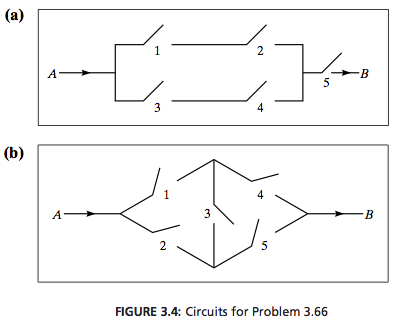
\includegraphics{p108_66}
  \begin{enumerate}[(a)]
    \item
      \begin{homeworkSection}{Solution}
        \[P(A) = p_5 (p_1 p_2 + p_3 p_4)\]
      \end{homeworkSection}
    \item
      \begin{homeworkSection}{Solution}
        \[P(B) = p_1 p_5 + p_1 p_3 p_5 + p_2 p_5 + p_2 p_3 p_4\]
      \end{homeworkSection}
  \end{enumerate}
\end{homeworkProblem}
%=============================p.173 5==========================% 
\newpage
\begin{homeworkProblem}
  Let $X$ represent the difference between the number of heads
  and the number of tails obtained when a coin is tossed $n$ times. 
  What are the possible values of $X$?
  \begin{homeworkSection}{Solution}
    Assuming the absolute value to be taken of the difference and
    letting $i$ represent the possible values, then 

    \[0 \le i \le n\]

  \end{homeworkSection}
\end{homeworkProblem}
%=============================p.173 6==========================% 
\newpage
\begin{homeworkProblem}
In Problem 5, for $n = 3$, if the coin is assumed fair, what are 
the probabilities associated with the values that $X$ can take on?

  \begin{homeworkSection}{Solution}


  \end{homeworkSection}
\end{homeworkProblem}
\end{spacing}
\end{document}

\begin{comment}%==========================================================
%=============================Problemi==========================% 
\newpage
\begin{homeworkProblem}

  \begin{homeworkSection}{Solution}

  \end{homeworkSection}
\end{homeworkProblem}
%=============================Problemi==========================% 
\begin{homeworkProblem}

  \begin{enumerate}[(a)]
    \item 
      \begin{homeworkSection}{Solution}

      \end{homeworkSection}
  \end{enumerate}
\end{homeworkProblem}
\end{comment}

\begin{comment}
  ## Homework
Due Tuesday
* P.107 66
* P.173 5, 6, 21, 35, 37, 38
* P.180 6, 7, 8, 9
\end{comment}
